\chapter{Gigantes Plaki}
\label{ch:gigantes-plaki}
\index{salad}
\index{tomato}
\index{beans}
\textit{Lima beans in tomato sauce}

Family member: Elsa \& Vaski

\marginnote[20pt]{\\
    \textbf{Makes 6-8 servings} \\
    Prep time: 20 minutes \\
    Cook time: 2 hours + overnight soaking \\
    \vspace*{\baselineskip}
    
    500g gigantes (lima) beans, dried and soaked in cold water overnight \\
    1 medium onion, finely chopped \\
    4-5 tbsp parsley, chopped \\
    1/2 tsp celery, finely chopped \\
    1 garlic clove, minced \\
    1/2 cup olive oil \\
    1/4 cup hot water + 1/4 cup more if needed \\
    400g can diced tomatoes \\
    Pinch dried oregano \\
    Salt \& pepper to taste
}

\begin{marginfigure}
  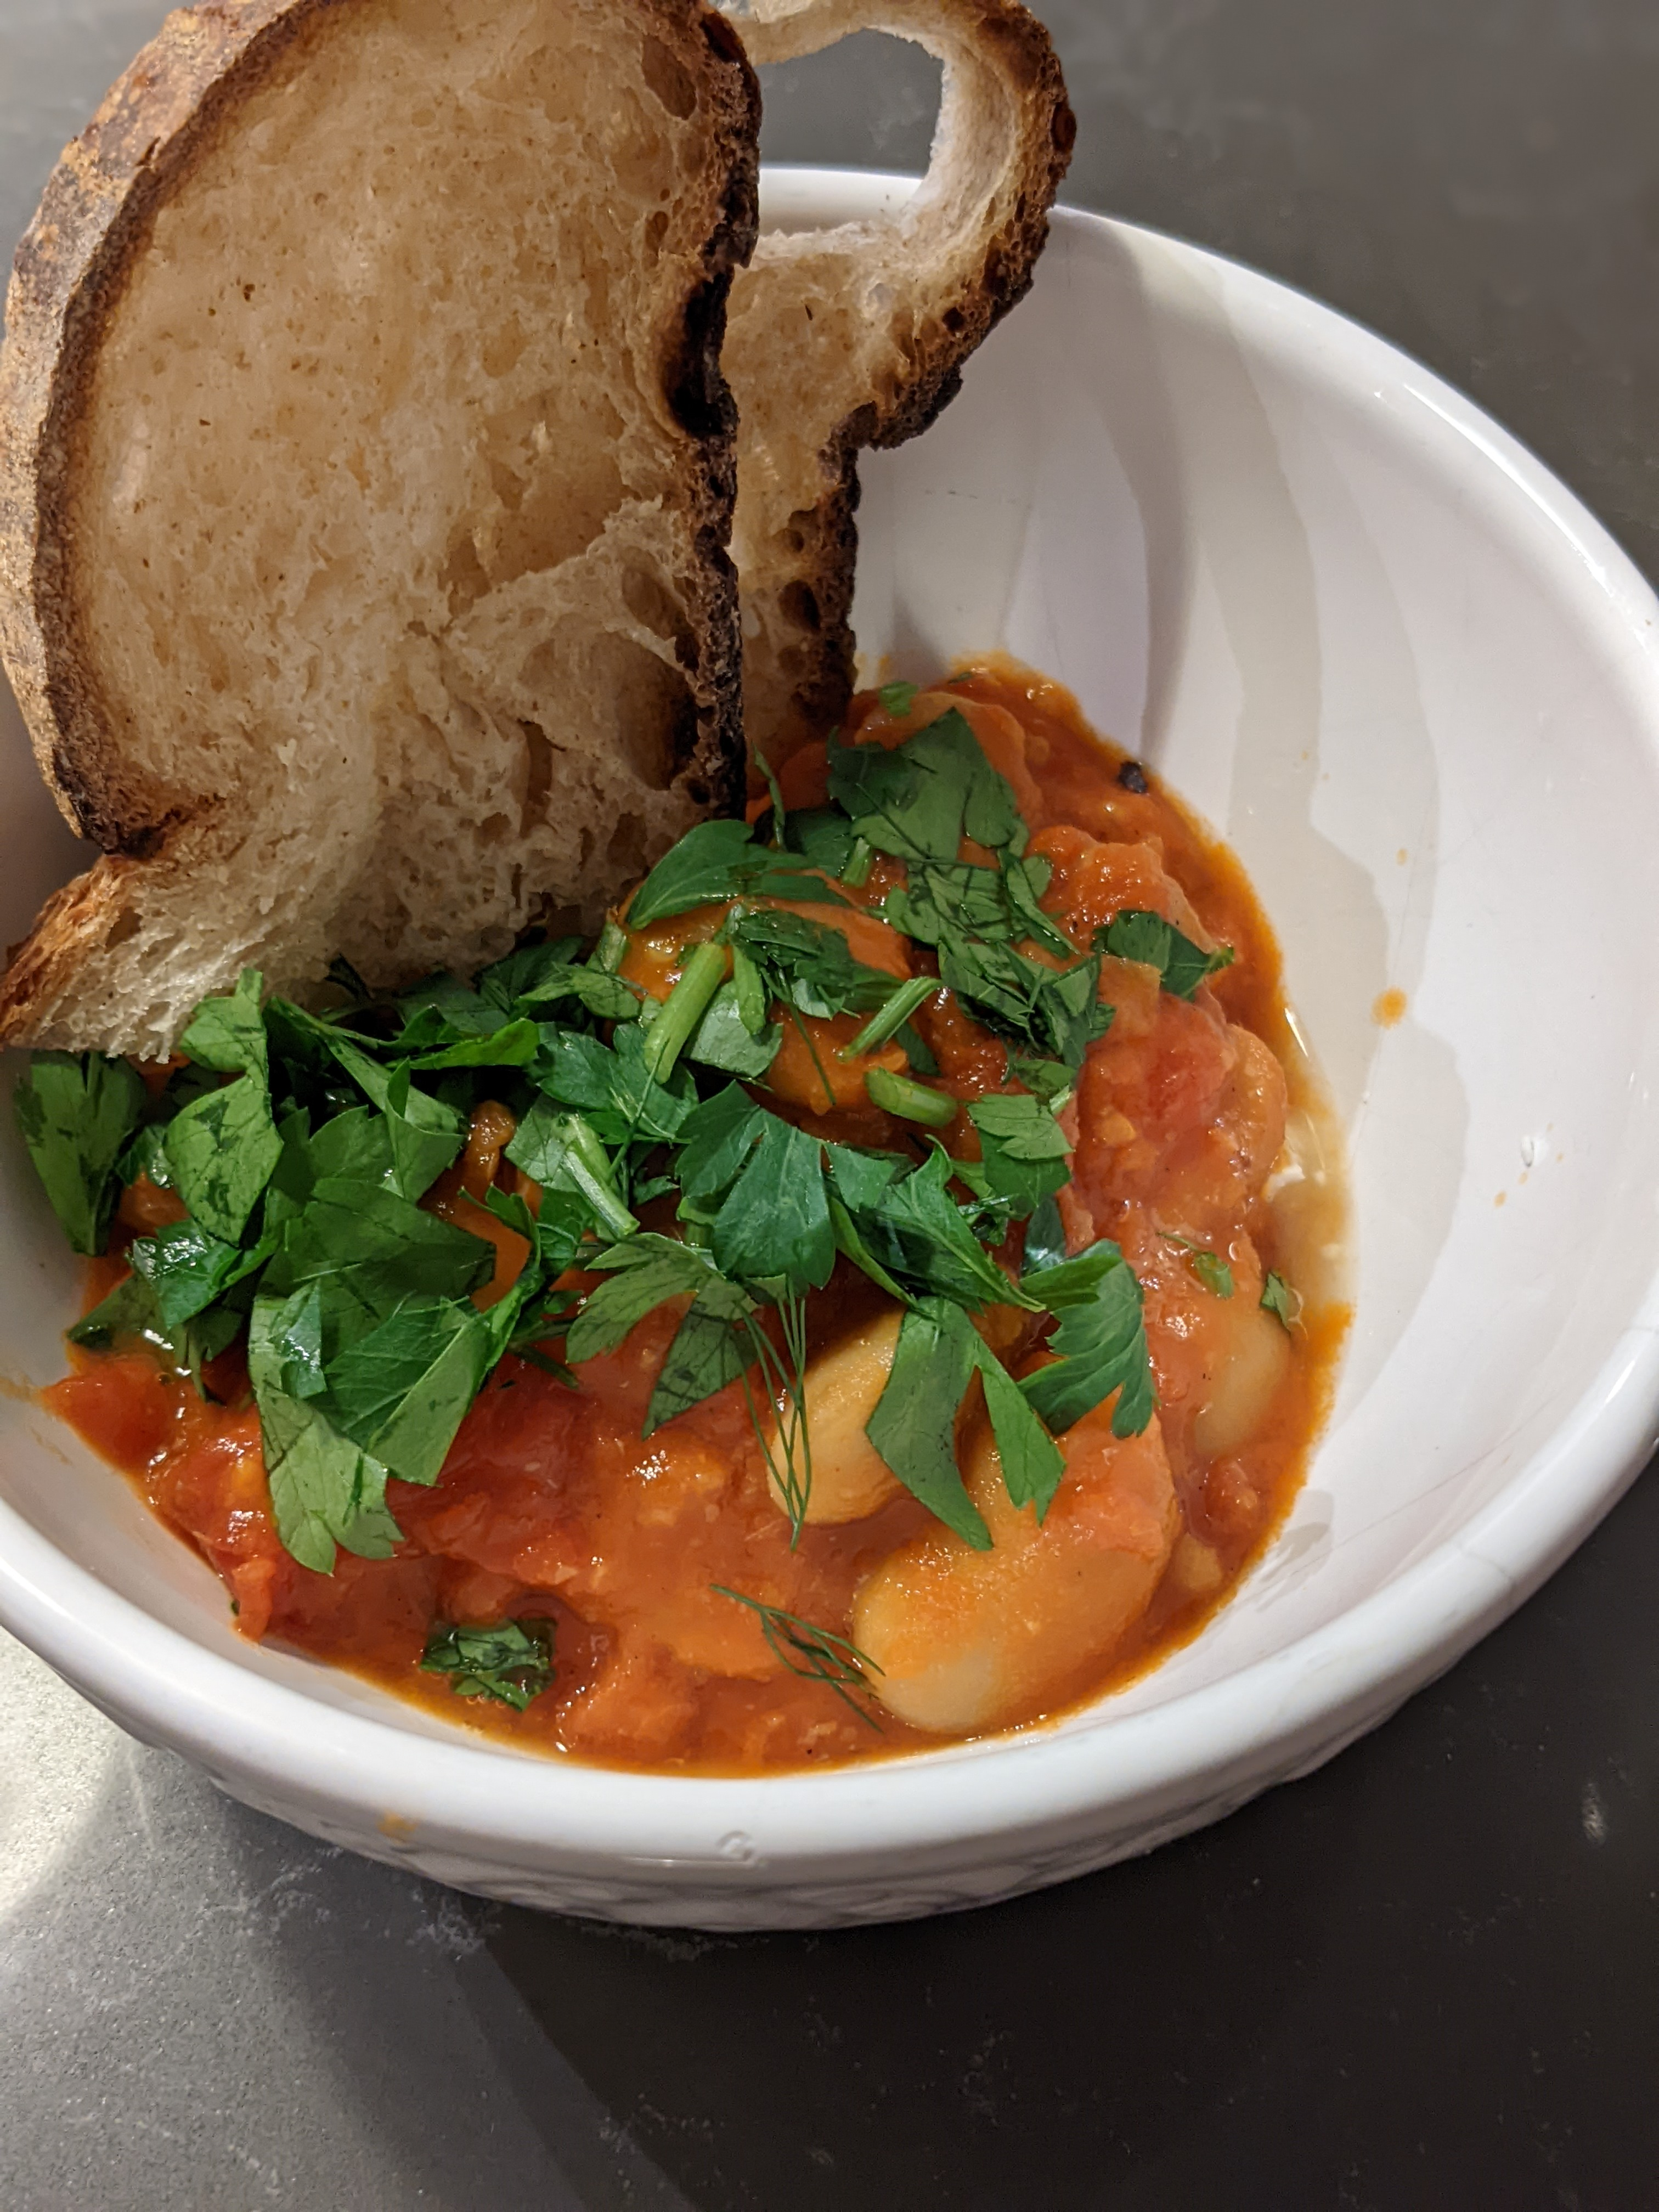
\includegraphics[width=60mm]{velsa/images/Gigantes.jpg}
\end{marginfigure}

\newthought{Who doesn't love} a bowl of gigantes plaki with a hearty sourdough bread and a generous slice of feta?

\bigskip

\begin{enumerate}
    \item Soak the gigantes beans in cold water overnight.
    \item The next day, drain the water.
    \item On the stove, heat olive oil in a large pot (or Creuset). Add the onion and cook until translucent. Add garlic and cook 1 minute more.
    \item Add the gigantes beans and hot water. Cook for about 30 minutes on the stove top.
    \item Add the diced tomatoes, parsley, celery (if using), oregano, salt and pepper. Place in the oven at 350\degree F.
    \item Simmer until reduced and thickened, and can add the 1/4 cup extra water to get wanted consistency.
    \item After about 1 hour, check peas for doneness, remove from oven and let cool.
    \item Top with more fresh parsley, serve with toasted village bread and feta.
\end{enumerate}

\marginnote{
    Do not over-stir the beans while cooking or will become mushy.
    Reminds me of Fassolada or Vaski's mom's beans.
}